\documentclass[tikz,border=6pt]{standalone}
% Shared style for the HERMESS schematic figures (compiled by build.sh).
% ETH palette; Latin Modern (the LaTeX default) to match the documentation.
\usepackage{amsmath}
\usepackage{tikz}
\usetikzlibrary{arrows.meta,positioning,calc,shapes.geometric,circuits.ee.IEC}
\definecolor{ethblue}{HTML}{215CAF}
\definecolor{ethpetrol}{HTML}{007894}
\definecolor{ethgrey}{HTML}{6F6F6F}
\tikzset{
  block/.style      = {draw=ethblue, thick, fill=ethblue!8, minimum height=9mm,
                       minimum width=16mm, inner sep=2.5pt, align=center},
  sum/.style        = {draw=ethblue, thick, circle, fill=white, minimum size=4.5mm, inner sep=0pt},
  sig/.style        = {-{Latex[length=2.4mm]}, thick},
  wire/.style       = {thick},
  node distance     = 9mm and 12mm,
  every node/.style = {font=\small},
  lbl/.style        = {font=\small, inner sep=1.5pt},
  port/.style       = {font=\small\itshape, text=ethgrey},
}

\begin{document}
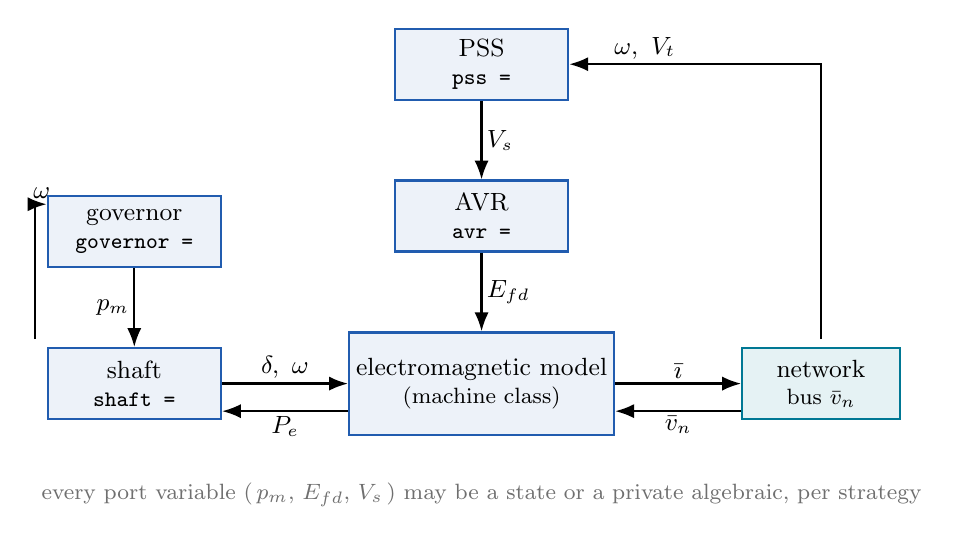
\begin{tikzpicture}[node distance=8mm and 14mm]
  \node[block, minimum width=30mm, minimum height=13mm] (em) {electromagnetic model\\[-1pt]{\footnotesize (machine class)}};
  \node[block, left=16mm of em, minimum width=22mm] (shaft) {shaft\\[-1pt]{\footnotesize\texttt{shaft =}}};
  \node[block, above=10mm of shaft, minimum width=22mm] (gov) {governor\\[-1pt]{\footnotesize\texttt{governor =}}};
  \node[block, above=10mm of em, minimum width=22mm] (avr) {AVR\\[-1pt]{\footnotesize\texttt{avr =}}};
  \node[block, above=10mm of avr, minimum width=22mm] (pss) {PSS\\[-1pt]{\footnotesize\texttt{pss =}}};
  \node[block, right=16mm of em, minimum width=20mm, fill=ethpetrol!10, draw=ethpetrol] (grid) {network\\[-1pt]{\footnotesize bus $\bar v_n$}};
  \draw[sig] (gov) -- (shaft) node[midway, left, lbl] {$p_m$};
  \draw[sig] (avr) -- (em) node[midway, right, lbl] {$E_{fd}$};
  \draw[sig] (pss) -- (avr) node[midway, right, lbl] {$V_s$};
  \draw[sig] (shaft) -- (em) node[midway, above, lbl] {$\delta,\ \omega$};
  \draw[sig] ($(em.west)+(0,-0.35)$) -- ($(shaft.east)+(0,-0.35)$) node[midway, below, lbl] {$P_e$};
  \draw[sig] (em) -- (grid) node[midway, above, lbl] {$\bar\imath$};
  \draw[sig] ($(grid.west)+(0,-0.35)$) -- ($(em.east)+(0,-0.35)$) node[midway, below, lbl] {$\bar v_n$};
  \draw[sig] (shaft.north west) ++(-0.15,0.1) |- ($(gov.west)+(0,0.35)$) node[pos=0.8, above, lbl] {$\omega$};
  \draw[sig] ($(grid.north)+(0,0.1)$) |- (pss.east) node[pos=0.85, above, lbl] {$\omega,\ V_t$};
  \node[lbl, text=ethgrey] at ($(em.south)+(0,-0.75)$)
    {\footnotesize every port variable (\,$p_m$, $E_{fd}$, $V_s$\,) may be a state or a private algebraic, per strategy};
\end{tikzpicture}
\end{document}
